\documentclass{article}

\usepackage{graphicx}
\usepackage{tikz}
\usepackage{tikzsymbols}
\usetikzlibrary{calc,patterns,shapes.geometric}
\pagestyle{empty}
\usepackage[margin=0pt]{geometry}
\geometry{papersize={14in,12in}}

\def\centerarc[#1](#2)(#3:#4:#5){\draw[#1] ($(#2)+({#5*cos(#3)},{#5*sin(#3)})$) arc (#3:#4:#5);}

\begin{document}
	\begin{figure}
		\centering
		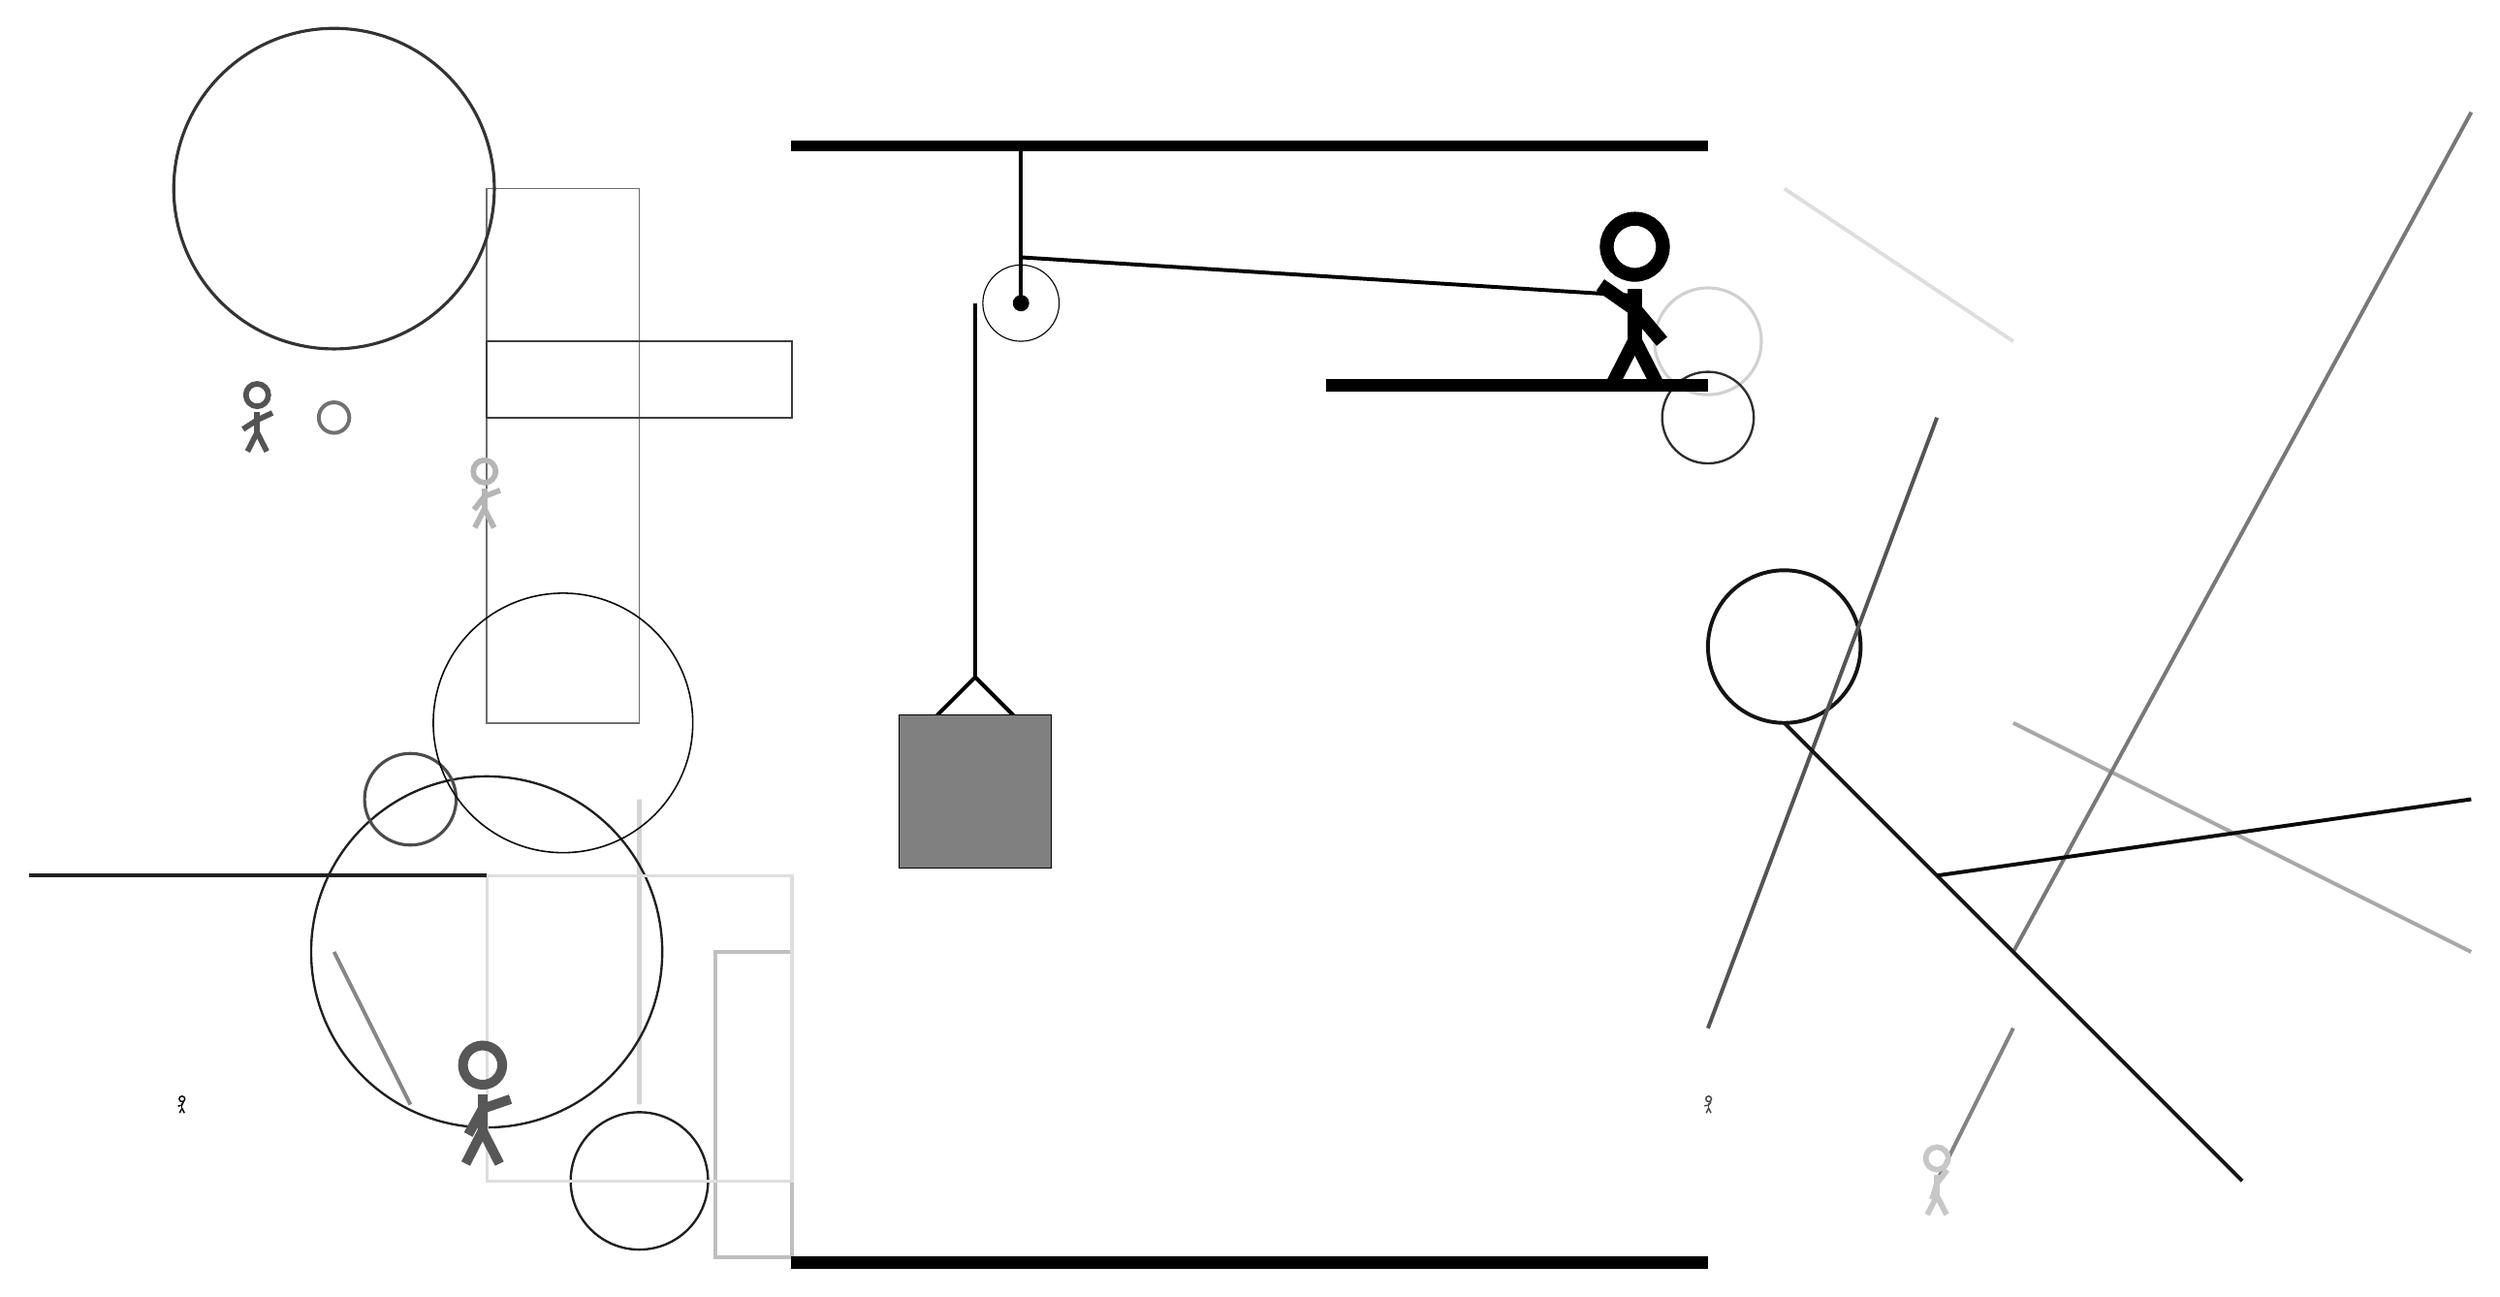
\begin{tikzpicture}
			%%%%% START %%%%%
			
			\draw[fill=black] (-2, 11.5) rectangle (10, 11.625);
			
			\draw[line width=0.7mm, color=black!17] (-4, 3) rectangle (-4, -1);
			
			\draw[line width=0.5mm, color=black!25] (-3, 1) rectangle (-2, -3);
			\draw [line width=0.3mm, color=black!88](-6, 1) circle (2.3);
			\draw[line width=0.2mm, color=black!57] (-4, 4) rectangle (-6, 11);
			\draw [line width=0.3mm, color=black!88](-4, -2) circle (0.9);
			\draw[line width=0.5mm, color=black!34](14, 4) -- (20, 1);
			\draw [line width=0.5mm, color=black!92](11, 5) circle (1.0);
			\draw[line width=0.5mm, color=black!53](14, 1) -- (20, 12);
			\draw[line width=0.4mm, color=black!13] (-2, 2) rectangle (-6, -2);
			\draw[line width=0.5mm, color=black!67](10, 0) -- (13, 8);
			\draw[line width=0.5mm, color=black!47](-7, -1) -- (-8, 1);
			\draw [line width=0.4mm, color=black!80](-8, 11) circle (2.1);
			\node[line width=0.7mm, color=black!29] at (-6, 7) {\Strichmaxerl[4][52][21]};
			\draw[line width=0.7mm, color=black!68] (12, -3) rectangle (12, -3);
			\draw [line width=0.5mm, color=black!56](-8, 8) circle (0.2);
			\draw[line width=0.5mm, color=black!13](14, 9) -- (11, 11);
			
			\node[line width=0.5mm, color=black!67] at (-9, 8) {\Strichmaxerl[4][33][25]};
			\draw [line width=0.4mm, color=black!70](-7, 3) circle (0.6);
			\node[line width=0.4mm, color=black!66] at (-6, -1) {\Strichmaxerl[7][61][19]};
			\draw[line width=0.5mm, color=black!91](11, 4) -- (17, -2);
			\draw [line width=0.4mm, color=black!18](10, 9) circle (0.7);
			
			\draw[line width=0.5mm, color=black!97](13, 2) -- (20, 3);
			\draw[line width=0.5mm, color=black!87](-6, 2) -- (-12, 2);
			\draw[line width=0.2mm, color=black!76] (-2, 9) rectangle (-6, 8);
			\node[line width=0.2mm, color=black!98] at (-10, -1) {\Strichmaxerl[1][14][68]};
			\draw[line width=0.5mm, color=black!49](13, -2) -- (14, 0);
			\draw [line width=0.3mm, color=black!82](10, 8) circle (0.6);
			\node[line width=0.3mm, color=black!73] at (10, -1) {\Strichmaxerl[1][10][55]};
			
			\node[line width=0.2mm, color=black!22] at (13, -2) {\Strichmaxerl[4][73][52]};
			
			\draw [line width=0.2mm, color=black!97](-5, 4) circle (1.7);
			
			\draw (1, 9.5) circle (0.5);
			\draw[fill=black] (1, 9.5) circle (0.1);
			\draw[line width=0.5mm] (1, 11.5) -- (1, 9.5);
			
			\draw[line width=0.5mm](-0.1, 4.1) --  (0.4, 4.6) -- (0.9, 4.1);
			\draw[fill=black!50] (-0.6, 4.1) rectangle (1.4, 2.1);
			
			\draw[line width=0.5mm](0.4, 9.5) -- (0.4, 4.6);
			\centerarc[line width=0.5mm](1, 9.5)(90:180:0.6)
			\draw[line width=0.5mm](1, 10.1) -- (9, 9.6);
			
			\node at (9, 9.5) {\Strichmaxerl[10][-35][-50]};
			\draw[fill=black] (5, 8.5) rectangle (10, 8.35);
			
			\draw[fill=black] (-2, -3) rectangle (10, -3.15);
			
			%%%%% END %%%%%
		\end{tikzpicture}
	\end{figure}	
\end{document}